
\de{ĐỀ THI HỌC KỲ I NĂM HỌC 2022-2023}{THPT Chuyên Lê Hồng Phong}


%==Bài 1==
\begin{bt}%[0T1B3-4]%[Dự án đề kiểm tra HKI NH22-23- Hiếu Mai]%[THPT Lê Hồng Phong]
Cho các tập hợp $ A=(-\infty;2) $, $ B=(-3;+\infty) $, $ C=(1;4) $. Tìm $ (A\cap B)\cup C $.\\
%\dapso{$ (-3;4) $}
\loigiai{
Ta thấy $ A \cap B = (-3;2) $ nên $ (A\cap B)\cup C = (-3;4) $.
}
\end{bt} 


%==Bài 2==
\begin{bt}%[0T2B2-3]%[Dự án đề kiểm tra HKI NH22-23- Hiếu Mai]%[THPT Lê Hồng Phong]
Biểu diễn miền nghiệm của hệ bất phương trình $ \heva{&x+y\leq 4\\&x\geq 1\\&y\geq 1} $ trên mặt phẳng $ Oxy $.
\loigiai{
\begin{center}
		\begin{tikzpicture}[line join=round, line cap=round,>=stealth,thick]
 			\tikzset{every node/.style={scale=0.9}}
 			\begin{scope}
 				\clip (-1,-1) rectangle (5,5);
 				\fill[pattern=north east lines] (-2,6)--(6,6)--(6,-2)--cycle;
 				\fill[pattern=north east lines] (1,-1)--(-1,-1)--(-1,5)--(1,5)--cycle;
 				\fill[pattern=north east lines] (-1,1)--(-1,-1)--(5,-1)--(5,1)--cycle;
 				\draw (-1,5)--(5,-1) node [pos=0.45, above, sloped] {$x + y - 4 = 0$};
 				\draw (1,-1)--(1,5) node [pos=0.45, above, sloped] {$x - 1= 0$};
 				\draw (-1,1)--(5,1) node [pos=0.45, below, sloped] {$y - 1= 0$};
 			\end{scope}
 			\draw[->] (-1,0)--(5,0) node[right]{$x$};
 			\draw[->] (0,-1)--(0,5) node[above]{$y$};
 			\draw (0,0) node[below left]{$O$};
 			\foreach \x in {1,4}{
 				\draw[thin] (\x,1pt)--(\x,-1pt) node [below] {$\x$};
			}
 			\foreach \y in {1,4}{
 				\draw[thin] (1pt,\y)--(-1pt,\y) node [left] {$\y$};
			}
 		\end{tikzpicture}
\end{center}
Vẽ và biểu diễn miền nghiệm (phần không bị gạch chéo) của từng bất phương trình trên mặt phẳng tọa độ $ Oxyz $. Phần còn lại không bị gạch bỏ là miền nghiệm của hệ bất phương trình đã cho.
}
\end{bt}

%==Bài 3==
\begin{bt}%[0T3B2-2]%[Dự án đề kiểm tra HKI NH22-23- Hiếu Mai]%[THPT Lê Hồng Phong]
Cho parabol $ (P)\colon y=x^2+ax+b $. Tìm $ a $, $ b $ biết $ (P) $ có trục đối xứng là $ d\colon x=2 $ và qua điểm $ A(0;3) $.
%\dapso{ $ a=-4 $; $ b=3 $}
\loigiai{
$ (P) $ có trục đối xứng là $ d\colon x=2 $ nên 
$$ \dfrac{-a}{2\cdot(1)} = 2 \Rightarrow a=-4 $$
Mặt khác, $ (P) $ đi qua điểm $ A(0;3) $ nên
$$
	3 = (0)^{2}-4(0)+b \Rightarrow b=3
$$
Vậy $ a=-4 $ và $ b=3 $.
}
\end{bt}
%==Bài 4==
\begin{bt}%[0T3B2-3]%[Dự án đề kiểm tra HKI NH22-23- Hiếu Mai]%[THPT Lê Hồng Phong]
	Cho hàm số $ f(x)=\heva{&x^2-4x+3&\text{khi}\,x\leq 3 \\&-x^2+10x-21&\text{khi}\,x>3.} $
	\begin{enumerate}
		\item Vẽ đồ thị hàm số $ f(x) $.
		\item Tìm tất cả các giá trị của tham số $ m $ sao cho phương trình $ f(x)=m $ có $ 2 $ phân biệt.
	\end{enumerate}
\loigiai{
\begin{enumerate}
\item Với $ x \le 3 $ thì đồ thị của hàm số $ f(x) $ có dạng parabol $ (P_{1}) \colon y=x^2-4x+3 $.
\\
Với $ x > 3 $ thì đồ thị của hàm số $ f(x) $ có dạng parabol $ (P_{2}) \colon y=-x^2+10x-21 $.
\\
Vẽ $ (P_{1}) $ với $ x\le 3 $ và $ (P_{2}) $ với $ x>3 $ trên cùng một hệ trục tọa độ, ta được đồ thị sau
\begin{center}
	\begin{tikzpicture}[line cap=butt,line join=miter,>=stealth]
	\tikzset{declare function={xmin=-1;xmax=8;ymin=-1.5;ymax=5;
					f(\x)=1*(\x)^2-4*(\x)+3; g(\x)=-1*(\x)^2+10*(\x)-21;
				},
				smooth,samples=450
			}
			\draw[->] (xmin,0)--(xmax,0) node[shift={(90:7pt)},font=\normalsize]{$ x $};
			\draw[->] (0,ymin)--(0,ymax) node[shift={(0:7pt)},font=\normalsize]{$ y $};
			\fill (0,0) node[below left,font=\normalsize]{$ O $};
			
			\clip (xmin,ymin) rectangle (xmax,ymax);
			\draw[dashed] (2,0)--(2,-1)--(0,-1) (5,0)--(5,4)--(0,4)
			;
			\draw[thin] (1,1pt)--(1,-1pt) node [below] {$1$};
			\draw[thin] (2,1pt)--(2,-1pt) node [above] {$2$};
			\draw[thin] (3,1pt)--(3,-1pt) node [below] {$3$};
			\draw[thin] (5,1pt)--(5,-1pt) node [below] {$5$};
			\draw[thin] (7,1pt)--(7,-1pt) node [below left] {$7$};
			\draw[thin] (1pt,-1)--(-1pt,-1) node [below left] {$-1$};
			\draw[thin] (1pt,3)--(-1pt,3) node [left] {$3$};
			\draw[thin] (1pt,4)--(-1pt,4) node [above right] {$4$};
			\draw[thick]  plot[domain=-1:3] (\x, {f(\x)});
			\draw[thick]  plot[domain=3:7.5] (\x, {g(\x)});
	\end{tikzpicture}
\end{center}
	\item $ f(x)=m $ là phương trình hoành độ giao điểm của đồ thị hàm số $ (C):y=f(x) $ và đường thẳng $ \Delta \colon y=m $. Để phương trình $ f(x)=m $ có $ 2 $ nghiệm phân biệt thì $ (C) $ cắt $ \Delta $ tại $ 2 $ điểm phân biệt. Dựa vào hình vẽ ta thấy $ m=-1 $ hoặc $ m=4 $ thỏa yêu cầu bài toán.
	\begin{center}
	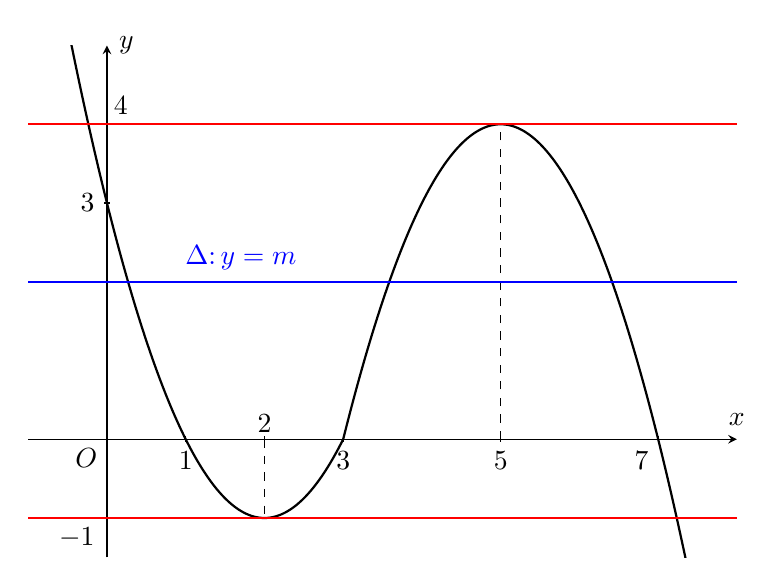
\begin{tikzpicture}[line cap=butt,line join=miter,>=stealth]
	\tikzset{declare function={xmin=-1;xmax=8;ymin=-1.5;ymax=5;
					f(\x)=1*(\x)^2-4*(\x)+3; g(\x)=-1*(\x)^2+10*(\x)-21;
				},
				smooth,samples=450
			}
			\draw[->] (xmin,0)--(xmax,0) node[shift={(90:7pt)},font=\normalsize]{$ x $};
			\draw[->] (0,ymin)--(0,ymax) node[shift={(0:7pt)},font=\normalsize]{$ y $};
			\fill (0,0) node[below left,font=\normalsize]{$ O $};
			
			\clip (xmin,ymin) rectangle (xmax,ymax);
			\draw[dashed] (2,0)--(2,-1)--(0,-1) (5,0)--(5,4)--(0,4)
			;
			\draw[thin] (1,1pt)--(1,-1pt) node [below] {$1$};
			\draw[thin] (2,1pt)--(2,-1pt) node [above] {$2$};
			\draw[thin] (3,1pt)--(3,-1pt) node [below] {$3$};
			\draw[thin] (5,1pt)--(5,-1pt) node [below] {$5$};
			\draw[thin] (7,1pt)--(7,-1pt) node [below left] {$7$};
			\draw[thin] (1pt,-1)--(-1pt,-1) node [below left] {$-1$};
			\draw[thin] (1pt,3)--(-1pt,3) node [left] {$3$};
			\draw[thin] (1pt,4)--(-1pt,4) node [above right] {$4$};
			\draw[thick]  plot[domain=-1:3] (\x, {f(\x)});
			\draw[thick]  plot[domain=3:7.5] (\x, {g(\x)});
			\draw[blue, thick] (-1,2)--(8,2) node[pos=.3, shift={(90:.3)}] {$ \Delta \colon y=m$};
			\draw[red, thick] (-1,-1)--(8,-1);
			\draw[red, thick] (-1,4)--(8,4);
	\end{tikzpicture}
\end{center}
\end{enumerate}
}
\end{bt}



%==Bài 5==
\begin{bt}%[0T4B1-2] [Dự án đề kiểm tra HKI NH22-23- Nguyen Huynh]%[Lê Hồng Phong]
	Cho $ 90^\circ<\alpha<180^\circ $	và $ \sin\alpha=\dfrac{12}{13} $. Tính $ \cos\alpha $, $ \tan\alpha $, $ \cot\alpha $.
	%\dapso{$ \cos\alpha =-\dfrac{5}{13}$; $ \tan\alpha =-\dfrac{12}{5}$;  $ \cot\alpha =-\dfrac{5}{12}$}
	\loigiai{Do $\cos^2\alpha+\sin^2\alpha=1$ nên $\cos^2\alpha=1-\left(\dfrac{12}{13} \right)^2=\dfrac{25}{169}$. 
		\\Mà $ 90^\circ<\alpha<180^\circ $ nên $\cos\alpha<0$. Vì vậy $\cos\alpha=-\dfrac{5}{13}$.\\
		Khi đó, $ \tan\alpha =\dfrac{\sin\alpha}{\cos\alpha}=-\dfrac{12}{5}$;  $ \cot\alpha =\dfrac{\cos\alpha}{\sin\alpha}=-\dfrac{5}{12}$. }
\end{bt}
%==Bài 6==
\begin{bt}%[0T5B3-2][Dự án đề kiểm tra HKI NH22-23- Nguyen Huynh]%[Lê Hồng Phong]
	Cho hình thang $ ABCD $ có $ \widehat{A}=\widehat{B}=90^\circ $, $ BC=a $, $ AD=2a $.
	\begin{enumerate}
		\item Chứng minh $ \overrightarrow{AC} = \overrightarrow{AB}+\dfrac{1}{2} \overrightarrow{AD}$.
		\item Gọi $ G $ là trong tâm tam giác $ ACD $. Tính $ AB $ theo $ a $ biết $ AG\perp BD $.
	\end{enumerate}
	%\dapso{$ AB=a $ }
	\loigiai{\begin{center}
			\begin{tikzpicture}
				\path 	(0:0) coordinate (A)
				++(90:3) coordinate (B)
				++(0:1) coordinate (C)
				($(A)+(0:2)$) coordinate (D)
				($(D)!0.5!(A)$) coordinate (C')
				($(D)!0.5!(C)$) coordinate (A')
				(intersection of A--A' and C--C') coordinate (G);%giao điểm O
				\draw (A)--(B)--(C)--(D)--cycle (C)--(A)--(G) (B)--(D);
				\foreach 	\x/ \goc in {A/180,B/180,C/0,D/0,G/-90} 
				\fill (\x) circle (1.5pt)
				($(\x)+(\goc:3mm)$) node {$\x$};
			\end{tikzpicture}
			
		\end{center}
		\begin{enumerate}
			\item Ta có $BC\parallel AD$ và $BC=\dfrac{1}{2}AD$ nên $\overrightarrow{BC}=\dfrac{1}{2}\overrightarrow{AD}$.\\
			Khi đó $\overrightarrow{AC}=\overrightarrow{AB}+\overrightarrow{BC}=\overrightarrow{AB}+\dfrac{1}{2}\overrightarrow{AD}$.
			\item Vì $AG\bot BD$ nên $\overrightarrow{AG}\cdot\overrightarrow{BD}=0$
			\[\begin{array}{l}
				\Leftrightarrow \dfrac{1}{3}\left(\overrightarrow{AC}+\overrightarrow{AD}\right)\left(\overrightarrow{AD}-\overrightarrow{AB}\right)=0\\
				\Leftrightarrow \left(\overrightarrow{AB}+\dfrac{3}{2}\overrightarrow{AD}\right)\left(\overrightarrow{AD}-\overrightarrow{AB}\right)=0\\
				\Leftrightarrow \dfrac{3}{2}AD^2-AB^2=0\;\left(\text{vì } \overrightarrow{AB}\cdot\overrightarrow{AD}=0\right)\\
				\Leftrightarrow AB=\dfrac{\sqrt{6}}{2}AD\\
				\Leftrightarrow AB=a\sqrt{6}\\
			\end{array}\]
		\end{enumerate}
	}
\end{bt}


%==Bài 7==
\begin{bt}%[0T4G2-2][Dự án đề kiểm tra HKI NH22-23- Nguyen Huynh]%[Lê Hồng Phong]
	Cho tam giác $ ABC $ nội tiếp đường tròn $ (O,R) $, phân giác trong góc $ A $ cắt đường tròn tại $ D $ ($ D $ khác $ A $). Biết $ \widehat{A}=75^\circ $, $ \widehat{B}=45^\circ $, tính tỉ số diện tích tam giác $ ABD $ và tam giác $ ACD $.
	%\dapso{$ \dfrac{\sqrt{3}}{\sqrt{2}} $ }
	\loigiai{\begin{center}
			\begin{tikzpicture}
				\tkzDefPoints{0/0/B,4/0/C}
				\tkzDefShiftPoint[B](45:3.6){A}
				\tkzDefLine[bisector](B,A,C)
				\tkzGetPoint{i}
				\tkzInterLL(A,i)(C,B) \tkzGetPoint{I}
				\tkzDefCircle[circum](A,B,C)
				\tkzGetPoint{O}
				\tkzDrawCircle(O,A)
				\tkzInterLC(A,I)(O,A)
				\tkzGetFirstPoint{D}
				\tkzDrawPoints(A,B,C,D,I,O)
				\tkzDrawSegments(A,D B,D C,D)
				\tkzDrawPolygon(A,B,C)
				\tkzLabelPoint[above](A) {$ A $}
				\tkzLabelPoint[left](B) {$ B $}
				\tkzLabelPoint[left](O) {$ O $}
				\tkzLabelPoints(I,C,D)
				\tkzMarkAngle[size=0.7](B,A,D)
				\tkzMarkAngle[size=0.6](D,A,C)
			\end{tikzpicture}
		\end{center}
		Ta có $\widehat{A}+\widehat{B}+\widehat{C}=180^{\circ}\Rightarrow \widehat{C}=60^{\circ}$.\\
		Áp dụng định lí sin cho tam giác $ABC$, ta có
		$$\dfrac{AB}{\sin C}=\dfrac{AC}{\sin B}\Rightarrow \dfrac{AB}{AC}=\dfrac{\sin C}{\sin B}=\dfrac{\sqrt{6}}{2}$$
		Mặt khác: $\dfrac{S_{\Delta ABD}}{S_{\Delta ACD}}=\dfrac{\dfrac{1}{2}AB\cdot AD\cdot\sin \widehat{BAD}}{\dfrac{1}{2}AC\cdot AD\cdot\sin \widehat{CAD}}=\dfrac{AB}{AC}=\dfrac{\sqrt{6}}{2}$.}
\end{bt}


%==Bài 8==
\begin{bt}%[0T6B2-1][Dự án đề kiểm tra HKI NH22-23- Nguyen Huynh]%[Lê Hồng Phong]
	Điểm chuẩn vào lớp $ 10 $	của trường có điểm chuẩn cao nhất trong từng quận huyện ở Thành phố Hồ Chí Minh năm $ 2021-2022 $ như sau
	\begin{center}
		\begin{tabular}{|c|c|c|c|c|c|c|c|c|c|c|}
			\hline
			$ 24{,}1 $ &$ 25{,}3 $ &$ 20$& 25&$ 25{,}2 $ &$ 24{,}7 $ &$ 20{,}7 $ &$ 25{,}9 $&$ 23{,}5 $ &$ 22{,}4 $ &$ 22{,}9 $   \\
			\hline
			$ 25{,}8 $ & $ 24$ & $ 25{,}6 $& $ 26{,}3 $ & $ 25{,}3 $ & $ 21{,}4 $ &$ 18{,}8 $ &16 & $ 21{,}8 $&$ 25{,}1 $ &$ 18{,}9 $ \\
			\hline
		\end{tabular}
	\end{center}
	Tính số trung bình, tứ phân vị, mốt, độ lệch chuẩn, khoảng biến thiên, khoảng tứ phân vị và tìm các giá trị bất thường của mẫu số liệu trên.
	%\dapso{ a) $\overline{x}=23{,}123$; độ lệch chuẩn $ 2{,}737 $; }
	\loigiai{Ta có dãy các giá trị từ bé đến lớn như sau 
		$$16;\,18{,}8;\,18{,}9;\, 20;\, 20{,}7;\,21{,}4;\, 21{,}8;\,22{,}4;\,22{,}9;\,23{,}5;\,24;$$$$24{,}1;\,24{,}7;\,25;\, 25{,}1;\,25{,}2;\,25{,}3;\,25{,}3;\,25{,}6;\,25{,}8;\,25{,}9;\,26{,}3.$$
		Ta có 
		\begin{itemize}
			\item Giá trị trung bình là $\overline{x}=23{,}123$.
			\item Tứ phân vị $Q_1=21{,}4;\,M_e=Q_2=24{,}05;\, Q_3=25{,}3$.
			\item Mốt $M_o=25{,}3$.
			\item  Độ lệch chuẩn $ 2{,}737 $.
			\item Khoảng biến thiên $R=10{,}3$.
			\item Khoảng tứ phân vị $\Delta_Q=3{,}9$.
		\end{itemize}
		Ta có $Q_1-1,5\Delta_Q=15{,}55$ và $Q_3+1,5\Delta_Q=31,25$. Do đó, trong dãy đã cho không có giá trị bất thường.
	}
\end{bt}